\documentclass{beamer}
\usepackage{tikz}
\usetikzlibrary{positioning}
\usepackage{graphicx}
\usepackage{xcolor}
\usepackage{multirow}
\usepackage{diagbox}

\usepackage[spanish]{babel}
\usepackage{amsmath, amssymb}


\usetheme{default}

\title{Toma de Decisiones Secuenciales \\ y Aprendizaje por Refuerzo}
\author{Daniela Pucci de Farias}
\institute{Universidad Torcuato Di Tella}
\date{Clase 1}

\begin{document}

\frame{\titlepage}

%------------------------------------------------
\begin{frame}{Toma de decisiones secuenciales}
\begin{center}
\Large
¿Qué creen que significa?
\end{center}
\end{frame}

\begin{frame}{¿D\'onde se utiliza?}
\begin{itemize}

\item Ejemplos:
\begin{itemize}
\item precios dinámicos
\item decisiones de inversión
\item gestión de inventario
\item control de producción
\end{itemize}
\item<2-> Muchas decisiones importantes:
\begin{itemize}
\item se toman a lo largo del tiempo
\item est\'an sujetas a incertidumbre
\item tienen impacto sobre posibilidades y resultados futuros
\end{itemize}

\end{itemize}
\end{frame}

\begin{frame}{¿Qué se llevan de este curso?}
\begin{itemize}
\item Sin un buen marco:
\begin{itemize}
\item decisiones miopes
\item reglas ad hoc
\end{itemize}

\item<2-> En este curso van a aprender a:
\begin{itemize}
\item \textbf{estructurar} estos problemas
\item \textbf{evaluar} consecuencias futuras
\item \textbf{tomar decisiones de forma consistente}
\end{itemize}
\end{itemize}
\end{frame}

\begin{frame}{Contenidos del Curso}
\begin{itemize}
\item Modelado y resolución de problemas de toma de decisiones secuenciales
\begin{itemize}
\item<2-> Procesos markovianos de decisión
\item<2-> Aprendizaje por refuerzo
\end{itemize}
\item<3-> Cronograma:
\begin{itemize}
\item<4-> Clase 1: Introducción a toma de decisiones secuenciales y aprendizaje por refuerzo. Procesos markovianos. Aplicaciones al estudio de regímenes de mercado y análisis de participación de empresas en el mercado.

\item<5-> Clase 2: Procesos Markovianos con Recompensa y Procesos Markovianos de Decisión (MDP). MDPs con horizonte finito. Modelado y algoritmos. Aplicación a precificación dinámica.

\item<6-> Clase 3: MDPs con horizonte infinito. Modelado y algoritmos. Aplicación a optimización de portafolios.

\item<7-> Clase 4: Aprendizaje por refuerzo. Métodos computacionales exactos y por simulación.

\item<8-> Clase 5: Sistemas de larga escala. Métodos de aproximación. Aplicación a precificación de opciones americanas.
\end{itemize}
\end{itemize}   
\end{frame}

\begin{frame}{Horas de Consulta}
\begin{itemize}
\item Anteriormente a las clases teóricas, de 18 a 19h.
\item Ubicación:
\begin{itemize}
\item 2/6: Aula SV403 (4to piso, edificio Sáenz Valiente).
\item 9/6: Aula SV402 (4to piso, edificio Sáenz Valiente).
\item 23/6: Sala 4 (4to piso, edificio ALCORTA).
\item 30/6: Aula SV101 (1er piso, edificio Sáenz Valiente).
\item 7/7: Aula SV101 (1er piso, edificio Sáenz Valiente).
\end{itemize}
\end{itemize}
\end{frame}

\begin{frame}{Criterio de Evaluación}
La nota estará basada en el siguiente esquema de ponderación: 
\begin{itemize}
\item Participación en clase, asistencia y puntualidad: 10\%
\item<2-> Trabajo práctico grupal: 40\% 
\begin{itemize}
\item<3-> formación de los grupos: 9 de junio 
\item<3-> Propuesta de proyecto: 30 de junio
\item<3-> Presentación oral (15 minutos) y relatorio final: 31 de julio
\end{itemize}
\item<4-> Tareas individuales (2 tareas): 50\%
\begin{itemize}
\item<5-> Tarea 1: asignada el 2 de junio, fecha de entrega el 16 de junio
\item<5-> Tarea 2: asignada el 9 de junio, fecha de entrega el 23 de junio
\end{itemize}
\item<6-> Tareas y código python (Google Colab) deben ser entregados por el campus virtual
\end{itemize}
\end{frame}

\begin{frame}{Modelando Toma de Decisiones Secuenciales}
\begin{itemize}
\item<1-> Ejemplos:
\begin{itemize}
\item precios dinámicos
\item decisiones de inversión
\item gestión de inventario
\item control de producción
\item agentes que interactúan con un entorno
\end{itemize}
\item<2->Una pregunta:
\begin{center}
¿Cómo estructuramos estos problemas?
\end{center}
\item<3-> Idealmente:
\begin{center}
\Large
\textbf{un único marco que sirva para todos}
\end{center}
\end{itemize}
\end{frame}

\begin{frame}
\frametitle{Un Marco Para Toma de Decisiones Secuenciales}
 \centering
 \mode<beamer>{
    \only<1>{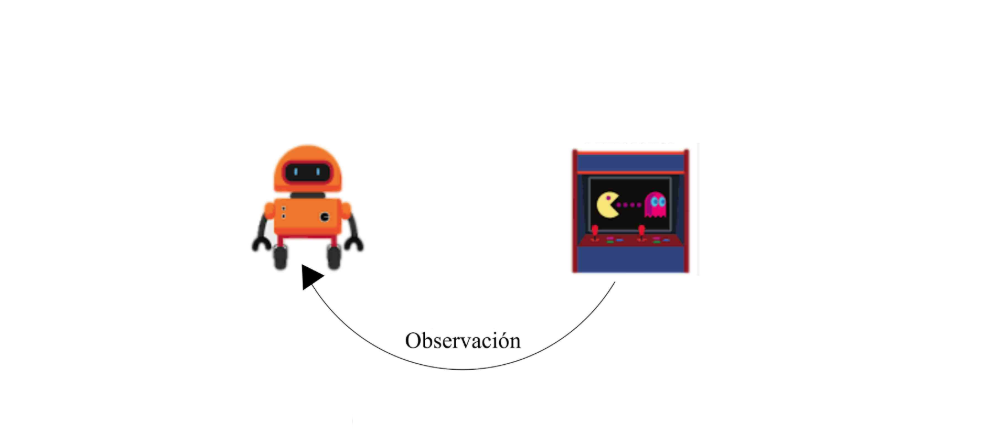
\includegraphics[width=1\textwidth]{../Images/RL/RL1.png}}
    \only<2>{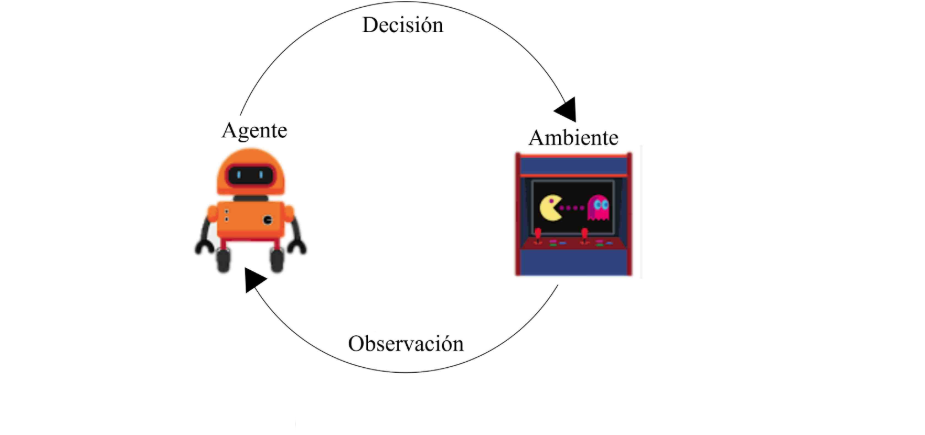
\includegraphics[width=1\textwidth]{../Images/RL/RL2.png}}}
    \only<3->{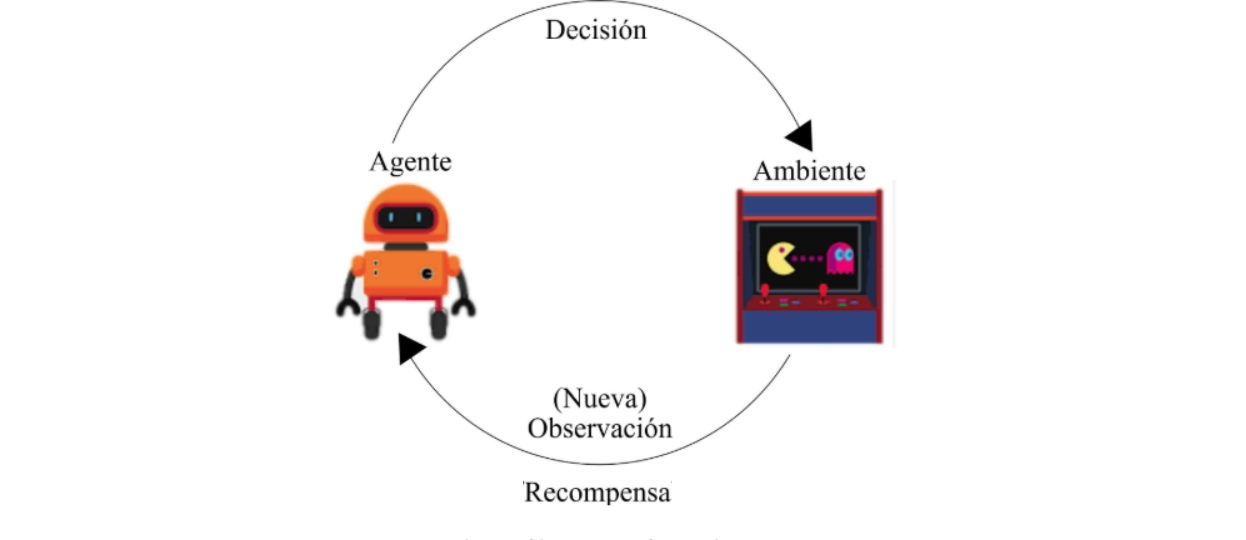
\includegraphics[width=1\textwidth]{../Images/RL/RL3_new.jpg}}
\only<4>{\textquestiondown C\'omo representar el problema matem\'aticamente?}
\end{frame}

\begin{frame}
\frametitle{Procesos Markovianos de Decisi\'on (MDPs)}
\begin{center}
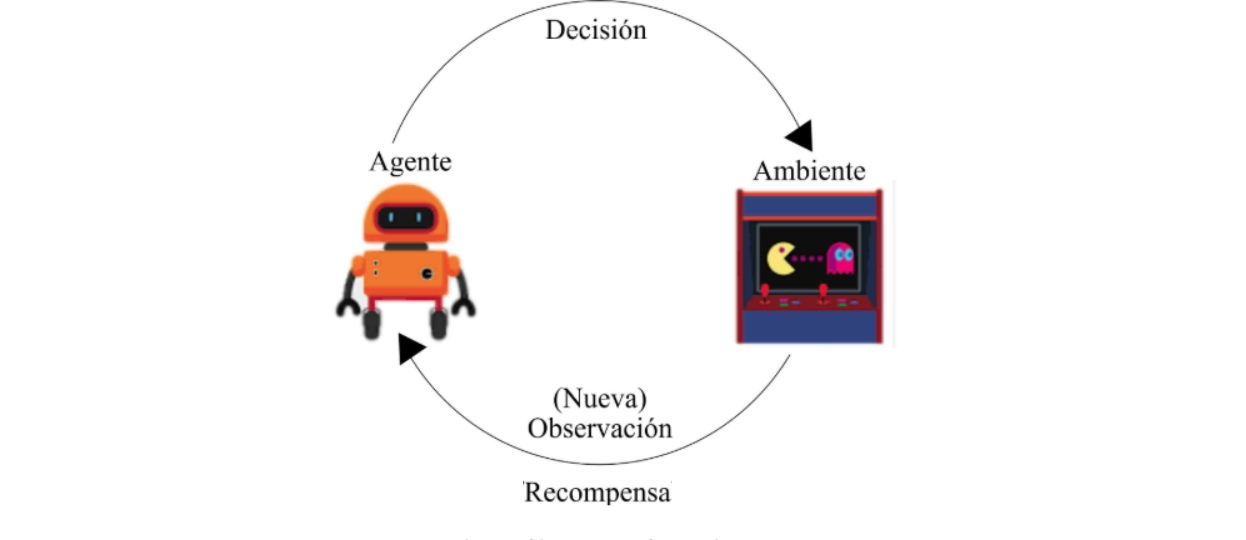
\includegraphics[width=0.8\textwidth]{../Images/RL/RL3_new.jpg}
\end{center}
\begin{itemize}
\item Componentes para un modelo de toma de decisiones secuenciales:
\begin{itemize}
    \item<2-> Ambiente tiene un \textbf{estado} que cambia al largo del tiempo 
    \item<3-> \textbf{Decisiones} son tomadas a partir de \textbf{observaciones}, que contienen informaci\'on parcial o total sobre el estado
    \item<4-> \textbf{Evolución del estado} afectada por decisiones e incertidumbre
    \item<5-> \textbf{Función de “recompensa”} afectada por estado y decisiones
\end{itemize}
\end{itemize}
\end{frame}

\begin{frame}
\frametitle{Procesos Markovianos de Decisi\'on (MDPs)}
\begin{center}
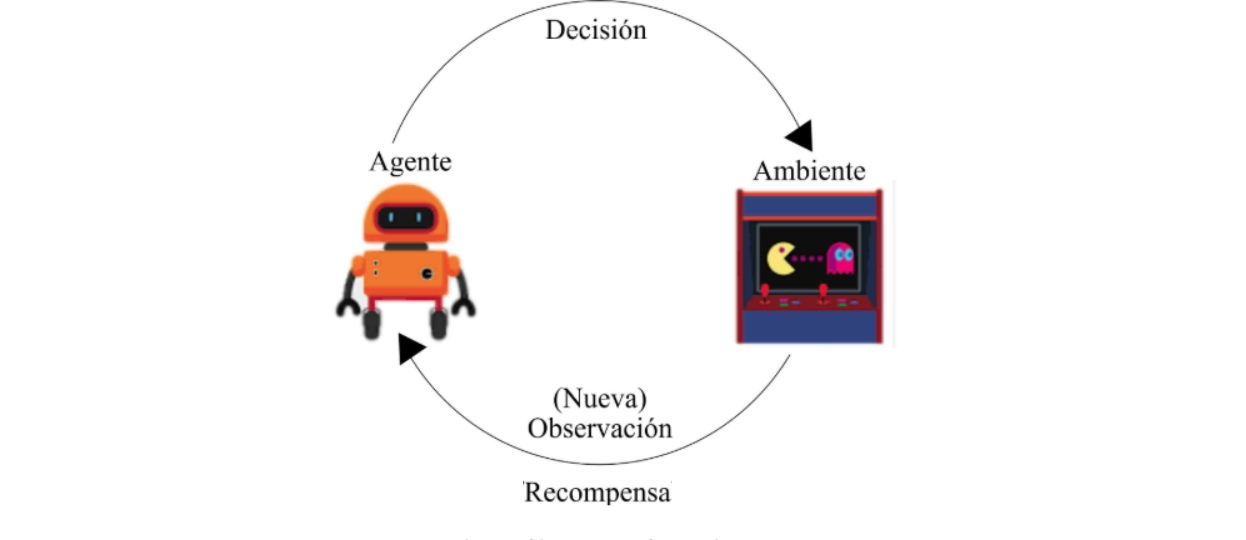
\includegraphics[width=0.8\textwidth]{../Images/RL/RL3_new.jpg}
\end{center}
\begin{itemize}
\item La función de recompensa puede ser diseñada para expresar diferentes objectivos
\item<2-> Toma de decisiones secuenciales: Desarrollo de estrategias óptimas para situaciones que se extienden en el tiempo, en ambientes sujetos a incertidumbre.
\begin{itemize}
\item Aprendizaje por refuerzo/reinforcement learning: toma de decisiones secuenciales donde aprendizaje se hace necesario por ausencia de modelo y/o complejidad del problema
\end{itemize}
\item<3-> Para formalizar la descripci\'on de MDPs, vamos a empezar con un \textbf{ambiente aut\'onomo}, y gradualmente agregar componentes hasta llegar a su definici\'on completa.
\end{itemize}
\end{frame}

%------------------------------------------------

%\begin{frame}{Ejercicio: Pensar en decisiones}
%\begin{itemize}
%\item Pensá en una decisión que:
%\begin{itemize}
%\item Se toma repetidamente
%\item Tiene incertidumbre
%\item Afecta el futuro
%\end{itemize}

%\item<2-> ¿Qué información te gustaría tener antes de decidir?

%\item<3-> Esa información resume la situación actual
%\end{itemize}
%\end{frame}

%------------------------------------------------

\begin{frame}{Modelando Un Ambiente Aut\'onomo}
\begin{itemize}
\item Ejemplo: cómo representar condiciones de mercado?
\item<2->En cada semana, uno de tres posibles estados
\item<3->Cómo evolucionan en el tiempo? 
\begin{itemize}
\item<4-> Descripción en términos de probabilidad
\item<6->En este curso, nos enfocaremos en procesos a tiempo discreto: \textbf{processos markovianos}
\end{itemize}
\end{itemize}
\centering
\mode<beamer>{
\only<2>{
\includegraphics[width=0.85\textwidth]{../Images/Market/Market1.png}}
\only<3>{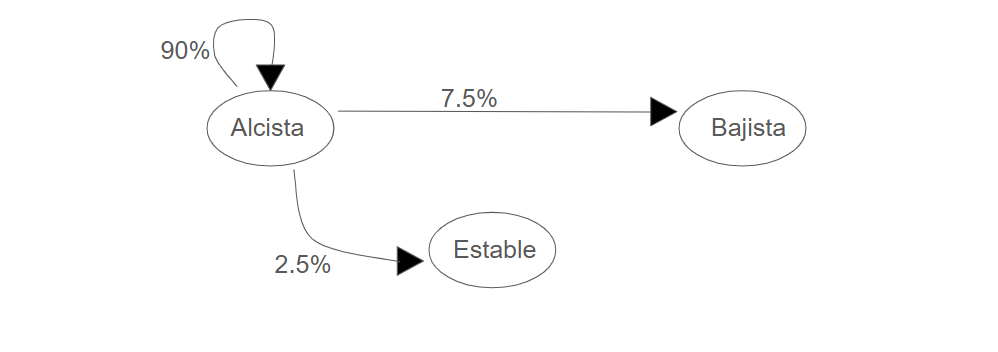
\includegraphics[width=0.85\textwidth]{../Images/Market/Market2.png}}
\only<4>{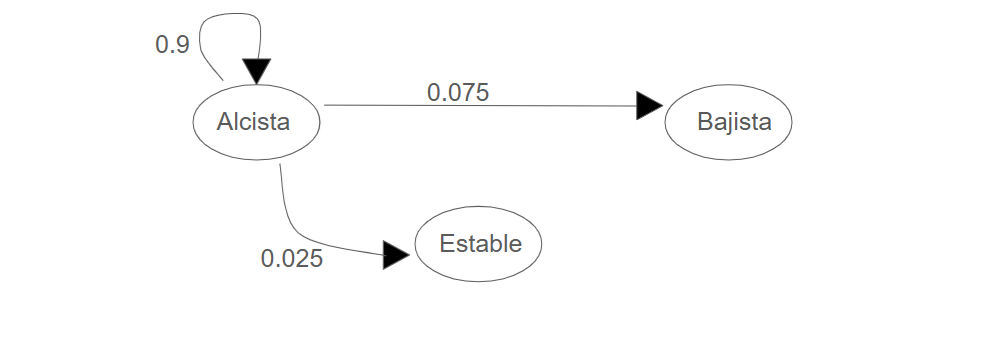
\includegraphics[width=0.85\textwidth]{../Images/Market/Market3.png}}
\visible<5->{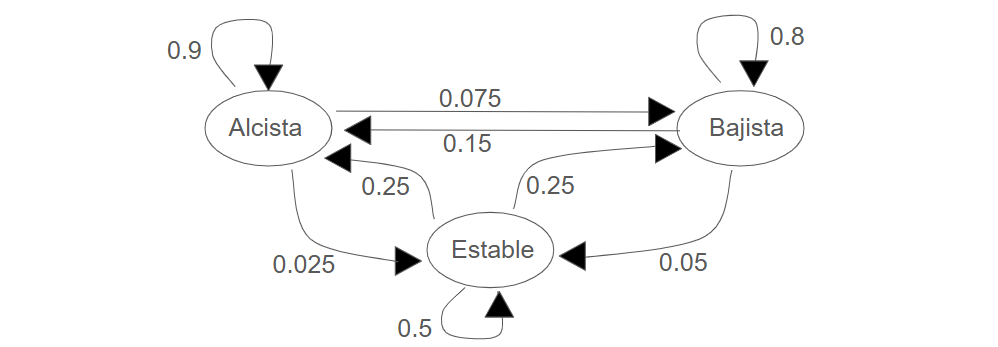
\includegraphics[width=0.85\textwidth]{../Images/Market/Market4.png}}}
\end{frame}

\begin{frame}{Procesos Markovianos}
Cómo definir matemáticamente el proceso de regímenes de mercado?
\begin{columns}[t]
\visible<2->{
\begin{column}[t]{0.6\textwidth}
\begin{itemize}
\item<2-> Espacio de estados $S$:
\begin{itemize}
    \item<2-> $S = \left\{\textbf{Alcista}, \textbf{Bajista}, \textbf{Estable}\right\}$
    \item<2-> Estados pueden ser discretos o continuos
\end{itemize}
\item<3-> Evolución en el tiempo
\mode<beamer>{
\only<3-7>{
\begin{tabular}{|c|c|c|c|}
\hline
    from/to & Alcista 2 & Bajista & Estable \\
    \hline
    Alcista & \visible<4-7>{0.9} &\visible<5-7>{0.075} & \visible<6-7>{0.025}  \\
    \hline
    Bajista & \visible<7>{0.15}&\visible<7>{0.8} & \visible<7>{0.05}  \\
    \hline
    Estable & \visible<7>{0.25}&\visible<7>{0.25} & \visible<7>{0.5} \\
    \hline    
\end{tabular}}}
\visible<8->{
\begin{itemize}
    \item Matriz de transición $P$: 
    $$P = \left[ 
    \begin{array}{ccc}
    0.9 & 0.075 & 0.025 \\
    0.15 & 0.8 & 0.05 \\
    0.25 & 0.25 & 0.5 \end{array}\right]$$
\end{itemize}}
\end{itemize}
\end{column}}
\begin{column}[t]{0.33\textwidth}
\mode<beamer>{
\only<1>{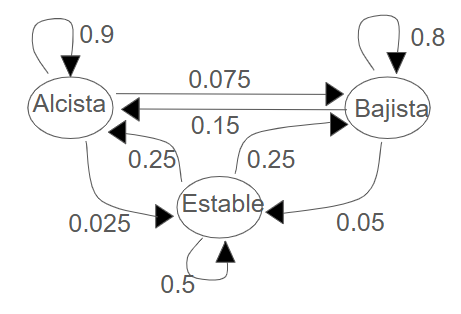
\includegraphics[width=1.1\textwidth]{../Images/MarkovProcess/MarkovProcess1.png}}
\only<2>{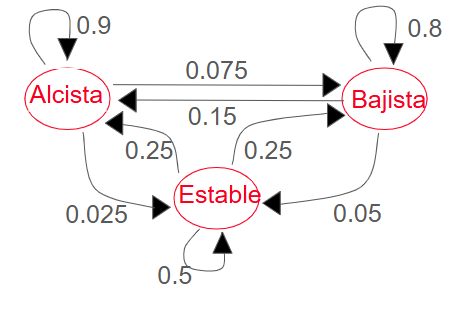
\includegraphics[width=1.1\textwidth]{../Images/MarkovProcess/MarkovProcess2.png}}
\only<3>{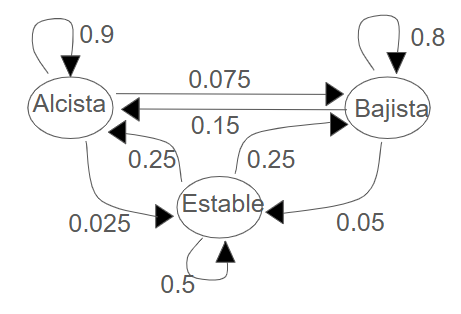
\includegraphics[width=1.1\textwidth]{../Images/MarkovProcess/MarkovProcess1.png}}
\only<4>{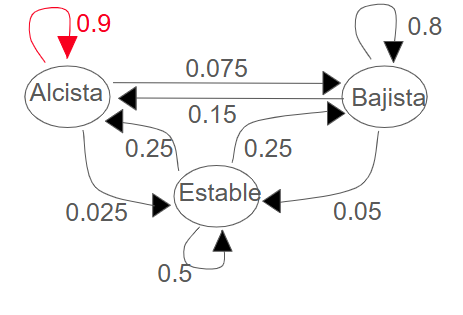
\includegraphics[width=1.1\textwidth]{../Images/MarkovProcess/MarkovProcess3.png}}
\only<5>{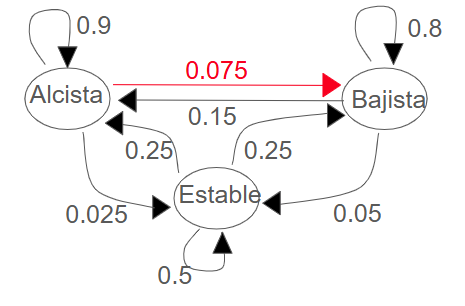
\includegraphics[width=1.1\textwidth]{../Images/MarkovProcess/MarkovProcess4.png}}
\only<6>{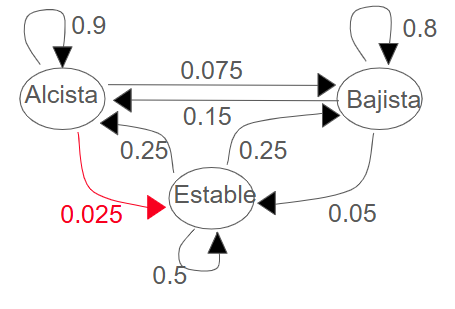
\includegraphics[width=1.1\textwidth]{../Images/MarkovProcess/MarkovProcess5.png}}}
\only<7->{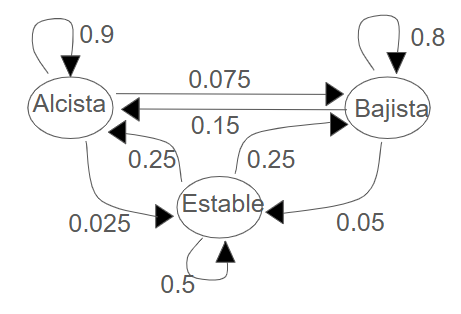
\includegraphics[width=1.1\textwidth]{../Images/MarkovProcess/MarkovProcess1.png}}
\end{column}
\end{columns}
\vspace{1em}
\visible<9->{
Tupla $(S,P)$ define el proceso markoviano
\begin{itemize}
    \item Si el número de estados es finito, también 
decimos cadena markoviana. 
\end{itemize}}
\end{frame}

\begin{frame}{Propiedad de Markov}
\begin{center}
\mbox{\hspace{-0.6cm}“El futuro del proceso markoviano depende solamente del estado presente.”}
\end{center}
\begin{itemize}
\item<2-> Proceso de Markov: tupla $(S,P)$
\item<3-> Estados  $s_0,~s_1,~s_2, \dots (s_t \in S ~{\rm for }~t = 0,1,2,\dots)$
\item<4-> ${\rm Prob}(s_{t+1}=s|s_0,s_1,...,s_t) = {\rm Prob}(s_{t+1}=s|s_t)$
\begin{itemize}
\item<5-> El estado st contiene toda la información relevante para el futuro del proceso
\item<5->Si conocemos $s_t$, podemos olvidar $s_{t-1}, ~s_{t-2},\dots,~s_0$.
\item<6->${\rm Prob}(s_{t+1}= s| s_t= s’) =   P(s,s’)$
\item<7-> Por ejemplo: 
$${\rm Prob}(s_{t+1}= \mathbf{Bajista} | s_t =\mathbf{Alcista}) = P(\mathbf{Alcista}, \mathbf{Bajista}) = 0.075$$
\end{itemize}
\end{itemize}
\end{frame}

\mode<beamer>{
\begin{frame}{Propiedad de Markov}
\begin{columns}[t]
\begin{column}[t]{0.6\textwidth}
\vspace{-2.5cm}
\only<1,2>{$$
\begin{array}{ccl} S & = & \left\{\textbf{Alcista}, \textbf{Bajista}, \textbf{Estable}\right\}\\
    P & = & \left[ 
    \begin{array}{ccc}
    0.9 & 0.075 & 0.025 \\
    0.15 & 0.8 & 0.05 \\
    0.25 & 0.25 & 0.5 \end{array}\right]
    \end{array}$$}
    \only<3>{$$
\begin{array}{ccl} S & = & \left\{\textbf{Alcista}, \textbf{Bajista}, \textbf{Estable}\right\}\\
    P & = & \left[ 
    \begin{array}{ccc}
    0.9 & \textcolor{red}{0.075} & 0.025 \\
    0.15 & 0.8 & 0.05 \\
    0.25 & 0.25 & 0.5 \end{array}\right]
    \end{array}$$}
\end{column}
\begin{column}{0.8\textwidth}
\only<1>{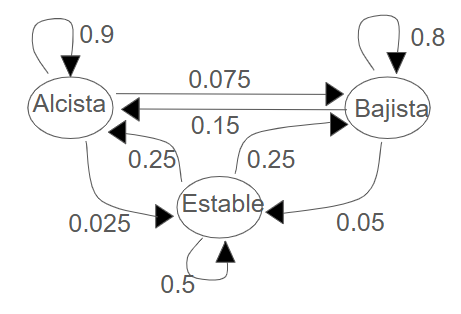
\includegraphics[width=0.4\textwidth]{../Images/MarkovProcess/MarkovProcess1.png}}
\only<2>{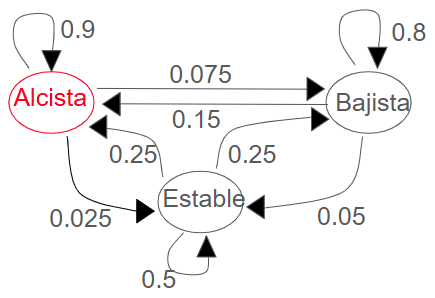
\includegraphics[width=0.4\textwidth]{../Images/MarkovProcess/MarkovProcess6.png}}
\only<3>{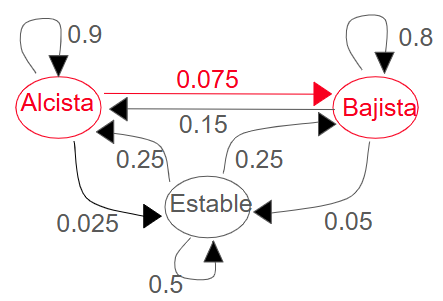
\includegraphics[width=0.4\textwidth]{../Images/MarkovProcess/MarkovProcess7.png}}
\end{column}
\end{columns}
Cuál es la probabilidad de tener un mercado \textbf {bajista en la próxima semana} 
\begin{enumerate} 
\item después de haber tenido un mercado \textbf {alcista en las últimas 5 semanas?}
\item después de haber tenido un mercado \textbf {alcista en la última semana, y bajista en las 4 anteriores?}
\end{enumerate}
\end{frame}}

\mode<handout>{
\begin{frame}{Propiedad de Markov}
\begin{columns}[t]
\begin{column}[t]{0.6\textwidth}
\vspace{-2.5cm}
    \only<3>{$$
\begin{array}{ccl} S & = & \left\{\textbf{Alcista}, \textbf{Bajista}, \textbf{Estable}\right\}\\
    P & = & \left[ 
    \begin{array}{ccc}
    0.9 & \textcolor{red}{0.075} & 0.025 \\
    0.15 & 0.8 & 0.05 \\
    0.25 & 0.25 & 0.5 \end{array}\right]
    \end{array}$$}
\end{column}
\begin{column}{0.8\textwidth}
\only<3>{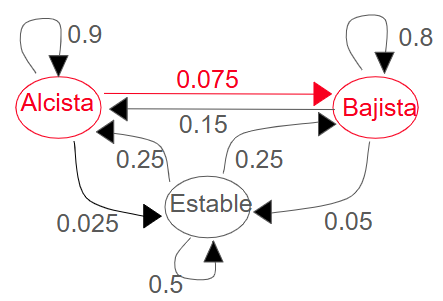
\includegraphics[width=0.4\textwidth]{../Images/MarkovProcess/MarkovProcess7.png}}
\end{column}
\end{columns}
Cuál es la probabilidad de tener un mercado \textbf {bajista en la próxima semana} 
\begin{enumerate} 
\item después de haber tenido un mercado \textbf {alcista en las últimas 5 semanas?}
\item después de haber tenido un mercado \textbf {alcista en la última semana, y bajista en las 4 anteriores?}
\end{enumerate}
\end{frame}}

\mode<beamer>{
\begin{frame}{Distribución Probabilística de Estados}
\begin{columns}[t]
\begin{column}[t]{0.6\textwidth}
\vspace{-2.5cm}
\only<1,3->{$$
\begin{array}{ccl} S & = & \left\{\textbf{Alcista}, \textbf{Bajista}, \textbf{Estable}\right\}\\
    P & = & \left[ 
    \begin{array}{ccc}
    0.9 & 0.075 & 0.025 \\
    0.15 & 0.8 & 0.05 \\
    0.25 & 0.25 & 0.5 \end{array}\right]
    \end{array}$$}
\only<2>{$$
\begin{array}{ccl} S & = & \left\{\textbf{Alcista}, \textbf{Bajista}, \textbf{Estable}\right\}\\
    P & = & \left[ 
    \begin{array}{ccc}
    0.9 & 0.075 & 0.025 \\
    0.15 & \textcolor{red}{0.8} & 0.05 \\
    0.25 & 0.25 & 0.5 \end{array}\right]
    \end{array}$$}
\end{column}
\begin{column}{0.8\textwidth}
\only<1,3->{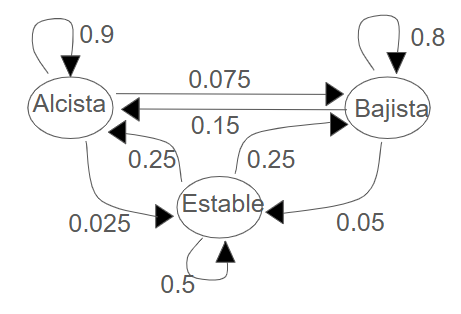
\includegraphics[width=0.4\textwidth]{../Images/MarkovProcess/MarkovProcess1.png}}
\only<2>{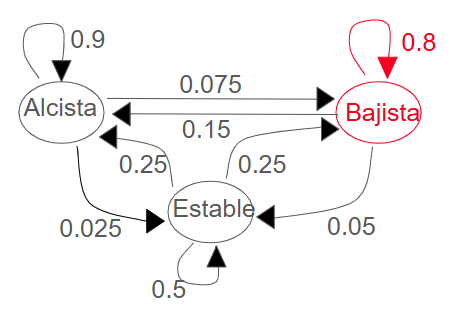
\includegraphics[width=0.4\textwidth]{../Images/MarkovProcess/MarkovProcess8.png}}
\end{column}
\end{columns}
\only<1>{Si esta semana el mercado es bajista, cuál es la probabilidad de que sea bajista en la próxima semana? En 2 semanas? En 10 semanas?}
\only<2>{Si esta semana el mercado es bajista, \textbf {cuál es la probabilidad de que sea bajista en la próxima semana?} En 2 semanas? En 10 semanas?}
\only<3-6>{Si esta semana el mercado es bajista, cuál es la probabilidad de que sea bajista en la próxima semana? \textbf{En 2 semanas?} En 10 semanas?}
\only<7,8>{Si esta semana el mercado es bajista, cuál es la probabilidad de que sea bajista en la próxima semana? En 2 semanas? \textbf{En 10 semanas?}}
\begin{itemize}
\only<2>{
\item La probabilidad de que sea bajista en la próxima semana es 0.8.}
\item<4-6> Podemos enumerar las posibilidades y sumarlas…
\only<5,6>{${\rm Prob}(\mathbf{Alcista}, \mathbf{Bajista}) + {\rm Prob}(\mathbf{Bajista}, \mathbf{Bajista}) + {\rm Prob}(\mathbf{Estable}, \mathbf{Bajista})$}
\only<6>{
	$ = 0.15*0.075 + 0.8*0.8 + 0.05*0.25$
    
	$= 0.66375$}
\item<8> Se puede responder a esas preguntas más fácilmente con álgebra linear!    
\end{itemize}
\end{frame}}

\mode<handout>{
\begin{frame}{Distribución Probabilística de Estados}
\begin{columns}[t]
\begin{column}[t]{0.6\textwidth}
\vspace{-2.5cm}
$$
\begin{array}{ccl} S & = & \left\{\textbf{Alcista}, \textbf{Bajista}, \textbf{Estable}\right\}\\
    P & = & \left[ 
    \begin{array}{ccc}
    0.9 & 0.075 & 0.025 \\
    0.15 & 0.8 & 0.05 \\
    0.25 & 0.25 & 0.5 \end{array}\right]
    \end{array}$$
\end{column}
\begin{column}{0.8\textwidth}
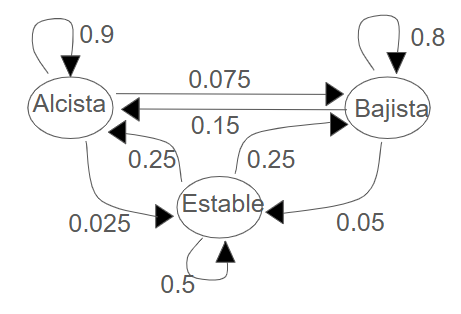
\includegraphics[width=0.4\textwidth]{../Images/MarkovProcess/MarkovProcess1.png}
\end{column}
\end{columns}
Si esta semana el mercado es bajista, cuál es la probabilidad de que sea bajista en la próxima semana? En 2 semanas? En 10 semanas?
\begin{itemize}
\item Se puede responder a esas preguntas más fácilmente con álgebra linear!    
\end{itemize}
\end{frame}}

\begin{frame}{Distribución Probabilística de Estados}

Vamos a representar una distribución probabilística de estados con la variable $\pi_t$: 

$$\pi_t(s) = {\rm Prob}(s_t = s).$$

\visible<2->{En nuestro ejemplo, si consideramos que esta semana corresponde a $t = 0$, tenemos ${\rm Prob}(s_0 = \mathbf{Altista}) = 0,~{\rm Prob}(s_0 = \mathbf{Bajista}) = 1),~{\rm Prob}(s_0 = \mathbf{Estable}) = 0.$}

\visible<3->{Entonces: 
$$
\pi_0 =\left[
\begin{array}{ccc}
0 & 1 & 0
\end{array}\right]$$}

\visible<4->{$\pi_0$ es la distribución inicial de estados en el proceso markoviano. } 
\visible<5>{
\begin{alertblock}{Resulta que $\pi_{t+1} = \pi_t P$  y  $\pi_t = \pi_0 P^t$.}
\end{alertblock}
}
\end{frame}

\begin{frame}{Distribución Probabilística de Estados}

Si esta semana el mercado es bajista, cuál es la probabilidad de que sea bajista en la próxima semana? En 2 semanas? En 10 semanas? 
\visible<2->{
\begin{alertblock}{Resulta que $\pi_t = \pi_0 P^t$.}
\end{alertblock}
}
\only<2>{
$$
\begin{array}{ccl}
\pi_1 & = & \pi_0 P \\
& = & \left[
\begin{array}{ccc}
0 & 1 & 0
\end{array}\right]\left[ 
    \begin{array}{ccc}
    0.9 & 0.075 & 0.025 \\
    0.15 & 0.8 & 0.05 \\
    0.25 & 0.25 & 0.5 \end{array}\right] \\
    & = & \left[\begin{array}{ccc}
0.15 & \textcolor{red}{0.8} & 0.05
\end{array}\right]
\end{array}$$
${\rm Prob}(s_1 = \textbf{Bajista}| s_0 = \textbf{Bajista}) = 0.8$
}
\only<3>{
$$
\begin{array}{ccl}
\pi_2 & = & \pi_0 P^2 \\
& = & \left[
\begin{array}{ccc}
0 & 1 & 0
\end{array}\right]\left[ 
    \begin{array}{ccc}
    0.9 & 0.075 & 0.025 \\
    0.15 & 0.8 & 0.05 \\
    0.25 & 0.25 & 0.5 \end{array}\right]^2 \\
    & = & \left[ \begin{array}{ccc}
0.2675 & \textcolor{red}{0.66375} & 0.06875
\end{array}\right]
\end{array}$$
${\rm Prob}(s_2 = \textbf{Bajista}| s_0 = \textbf{Bajista}) = 0.66375$
}
\only<4>{
$$
\begin{array}{ccl}
\pi_{10} & = & \pi_0 P^{10} \\
& = & \left[
\begin{array}{ccc}
0 & 1 & 0
\end{array}\right]\left[ 
    \begin{array}{ccc}
    0.9 & 0.075 & 0.025 \\
    0.15 & 0.8 & 0.05 \\
    0.25 & 0.25 & 0.5 \end{array}\right]^{10} \\
    & = & \left[ \begin{array}{ccc}
0.59159 & \textcolor{red}{0.34310} & 0.06532
\end{array}\right]
\end{array}$$
${\rm Prob}(s_10 = \textbf{Bajista}| s_0 = \textbf{Bajista}) = 0.34310$
}
\end{frame}

\begin{frame}{Distribución Probabilística de Estados}

Cuál es la frecuencia de semanas alcistas, bajistas y estables en ese mercado?

\visible<2->{Buscamos la \textbf{distribución estacionaria} de ese proceso.}
\begin{itemize}
    \item<3-> Tenemos $\pi_{t+1} = \pi_t x P$ y estacionariedad implica $\pi_{t+1} = \pi_t = \pi$.
    \item<4-> Queremos resolver \textcolor{red}{$\pi = \pi P$.}
    \item<5-> Si el número de estados es finito, siempre existe una solución, pero no es necesariamente única.
\end{itemize}
\visible<6->{
$$\begin{array}{ccl}
\pi_\infty & = & \pi_0 P^\infty \\
& = & \left[
\begin{array}{ccc}
0 & 1 & 0
\end{array}\right]\left[ 
    \begin{array}{ccc}
    0.9 & 0.075 & 0.025 \\
    0.15 & 0.8 & 0.05 \\
    0.25 & 0.25 & 0.5 \end{array}\right]^\infty \\
    & \approx & \left[ \begin{array}{ccc}
0.625 & \textcolor{red}{0.3125} & 0.0625
\end{array}\right]
\end{array}$$
}
\visible<7>{
\textbf{En ese mercado, 62.5\% de las semanas son alcistas, 31.25\% son bajistas, y 6.25\% son estables.}
}
\end{frame}
%\begin{frame}{Ejemplo: Google PageRank}
%Cuando hacemos una búsqueda en Google, las páginas que satisfacen a nuestras condiciones son presentadas en orden de importancia.

%Cómo determinar importancia/ranking?
%\mode<beamer>{
%\includegraphics<2>[width=1.1\textwidth]{../Images/PageRank/PageRank1.png}}
%\includegraphics<3>[width=1.1\textwidth]{../Images/PageRank/PageRank2.png}
%\end{frame}

\begin{frame}{Ejemplo: Participación en El Mercado}

Cadenas markovianas son frecuentemente utilizadas para modelar el comportamiento de usuarios de proveedores adversarios y predecir la participación en el mercado de esos proveedores al largo del tiempo.
\begin{itemize}
\item<2>$p_{ij} $= probabilidad que usuario de proveedor $i$ cambie a proveedor $j$ 
\end{itemize}
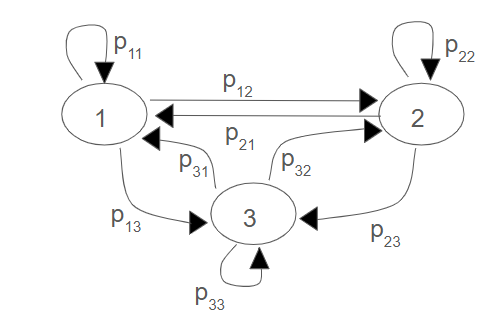
\includegraphics[width=0.8\textwidth]{../Images/RLExamples/MarketCompetition.png}
\end{frame}

\begin{frame}{Ejemplo: Participación en El Mercado}
\begin{center}
\textbf{Table 4: Respondents Brand Switching Behavior}
\only<1>{
\begin{tabular}{|c|c|c|c|c|c|c|c|}
\hline
\multirow{2}{*}{\textbf{Gains and Losses}} & \multicolumn{6}{|c|}{\textbf{Mobile Telecom Operators}} & \multirow{2}{*}{\textbf{Total}}  \\
&\textbf{M} & \textbf{V} & \textbf{T} & \textbf{E} & \textbf{A} & \textbf{G} & \\ \hline
\textbf{M} & 290 & 38 & 24 & 2 & 36 & 15 & \textbf{405} \\
\hline
\textbf{V} & 80 & 91 & 22 & 4 & 32 & 6 & \textbf{235} \\
\hline
\textbf{T} & 83 & 17 & 101 & 4 & 21 & 11 & \textbf{237} \\
\hline
\textbf{E} & 9 & 6 & 11 & 4 & 0 & 0 & \textbf{30} \\
\hline
\textbf{A} & 72 & 22 & 21 & 2 & 87 & 5 & \textbf{209} \\
\hline
\textbf{G} & 38 & 9 & 13 & 1 & 21 & 32 & \textbf{114} \\
\hline
\end{tabular}}
\mode<beamer>{
\only<2>{
\begin{tabular}{|c|c|c|c|c|c|c|c|}
\hline
\multirow{2}{*}{\textbf{Gains and Losses}} & \multicolumn{6}{|c|}{\textbf{Mobile Telecom Operators}} & \multirow{2}{*}{\textbf{Total}}  \\
&\textbf{M} & \textbf{V} & \textbf{T} & \textbf{E} & \textbf{A} & \textbf{G} & \\ \hline
\textbf{M} & 290 & 38 & 24 & 2 & 36 & 15 & \textcolor{red}{405} \\
\hline
\textbf{V} & 80 & 91 & 22 & 4 & 32 & 6 & \textcolor{red}{235} \\
\hline
\textbf{T} & 83 & 17 & 101 & 4 & 21 & 11 & \textcolor{red}{237} \\
\hline
\textbf{E} & 9 & 6 & 11 & 4 & 0 & 0 & \textcolor{red}{30} \\
\hline
\textbf{A} & 72 & 22 & 21 & 2 & 87 & 5 & \textcolor{red}{209} \\
\hline
\textbf{G} & 38 & 9 & 13 & 1 & 21 & 32 & \textcolor{red}{114} \\
\hline
\end{tabular}}
\only<3>{
\begin{tabular}{|c|c|c|c|c|c|c|c|}
\hline
\multirow{2}{*}{\textbf{Gains and Losses}} & \multicolumn{6}{|c|}{\textbf{Mobile Telecom Operators}} & \multirow{2}{*}{\textbf{Total}}  \\
&\textbf{M} & \textbf{V} & \textbf{T} & \textbf{E} & \textbf{A} & \textbf{G} & \\ \hline
\textbf{M} & 290 & \textcolor{red}{38} & 24 & 2 & 36 & 15 & \textcolor{red}{405} \\
\hline
\textbf{V} & 80 & 91 & 22 & 4 & 32 & 6 & \textbf{235} \\
\hline
\textbf{T} & 83 & 17 & 101 & 4 & 21 & 11 & \textbf{237} \\
\hline
\textbf{E} & 9 & 6 & 11 & 4 & 0 & 0 & \textbf{30} \\
\hline
\textbf{A} & 72 & 22 & 21 & 2 & 87 & 5 & \textbf{209} \\
\hline
\textbf{G} & 38 & 9 & 13 & 1 & 21 & 32 & \textbf{114} \\
\hline
\end{tabular}}}
{\textit{Source: Author's Computation (2013}}
\end{center}
\only<1>{“Prediction of Subscribers’ Brand Switching Behaviour and Ergodic Market Share of Network Service Providers in Ghana Using Markov Chain Model”, Ezekiel Nortey}
\begin{itemize}
\item<2->{Participación actual derivada de totales
\mode<beamer>{
$$
\begin{array}{ccl} \pi_0 & = & \left[\begin{array}{cccccc} 405 & 235 & 237 & 30 & 209 & 114\end{array}\right]/1230 \\
& = & \left[\begin{array}{cccccc} 0.33 & 0.19 & 0.19 & 0.02 & 0.17 & 0.09\end{array}\right]
\end{array}
$$}}

\item<3>{Matriz de transición $P$ derivada de la misma forma
\mode<beamer>{
\begin{itemize}
    \item Por ejemplo $P(M,V) = 38/405 = 0.094$.
\end{itemize}}}
\end{itemize}
\end{frame}


\begin{frame}{Ejemplo: Participación en El Mercado}

\begin{itemize}
\item Tenemos:
$$
\pi_0 = 
\left[
\begin{array}{cccccc}
0.329 & 0.191 & 0.193 & 0.024 & 0.170 & 0.093
\end{array}
\right]$$
$$
P = \left[
\begin{array}{cccccc}
0.716 & 0.094 & 0.059 & 0.005 & 0.089 & 0.037 \\
0.340 & 0.387 & 0.094 & 0.017 & 0.136 & 0.026 \\
0.350 & 0.072 & 0.426 & 0.017 & 0.089 & 0.046 \\
0.300 & 0.200 & 0.367 & 0.133 & 0.000 & 0.000 \\
0.344 & 0.105 & 0.100 & 0.010 & 0.416 & 0.024 \\
0.333 & 0.079 & 0.114 & 0.009 & 0.184 & 0.281 
\end{array}\right]
$$
\item<2> Analisamos el comportamiento de esa cadena markoviana en Python
\end{itemize}
\end{frame}

\begin{frame}{Ejemplo: Participación en El Mercado}
\centering
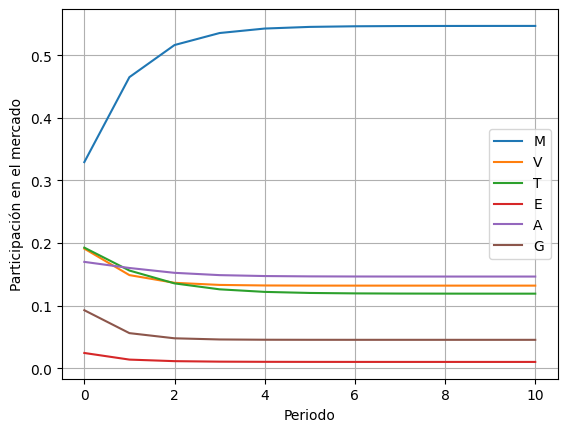
\includegraphics[width=1.0\textwidth]{../Images/RLExamples/MarketShare.png}
\end{frame}

\begin{frame}{La  Elecci\'on de Estado}
\begin{itemize}
\item Queremos describir cómo evoluciona el sistema

\item<2-> Definimos:
\begin{itemize}
\item \textbf{Estado}: resumen de la información relevante (propiedad de Markov)
\end{itemize}

\item<3-> Idea clave:
\begin{itemize}
\item El estado debe contener lo necesario para predecir el futuro
\end{itemize}

\item<4-> Si falta información:
\begin{itemize}
\item El modelo será incorrecto
\end{itemize}

\item<5-> Si hay informaci\'on redundante:
\begin{itemize}
\item El espacio de estados ser\'a m\'as largo del necesario, complejizando innecesariamente el tratamiento computacional del problema
\end{itemize}

\item<6-> En la pr\'actica, la elecci\'on del estado puede exijir tradeoffs entre captar la informaci\'on relevante y controlar la complejidad computacional.
\end{itemize}
\end{frame}

\begin{frame}{La  Elecci\'on de Estado}
\begin{itemize}
\item En el ejemplo de reg\'imenes de mercado, \textquestiondown qu\'e representa el estado que elijimos? Y \textquestiondown x\'omo puede fallar en la pr\'actica? 
\item<2-> Pensemos en otros ambientes con incertidumbre. \textquestiondown C\'omo modelarlos como process markovianos?
\end{itemize}
\end{frame}

\begin{frame}{Pero falta algo}
\begin{itemize}
\item Hasta ahora:
\begin{itemize}
\item Sabemos cómo evoluciona el sistema
\end{itemize}

\item<2-> Pero:
\begin{itemize}
\item No todos los estados son iguales
\end{itemize}

\item<3-> Necesitamos medir qué tan buenos son, seg\'un alg\'un criterio que nos interese
\end{itemize}
\end{frame}

\begin{frame}{Funci\'on de Recompensa}
\begin{itemize}
\item Para toma de decisiones, normalmente estamos interesados en uno o más objectivos:
\begin{itemize}
\item<2-> Maximizar ganancias
\item<3-> Minimizar costos
\item<4-> Ganar un juego, o cumplir con una meta
\item<5-> Minimizar riesgos
\item<6-> ???
\end{itemize}
\item<7-> Expresamos el objectivo a traves de la {\bf función de recompensa}
\end{itemize}
\end{frame}



\begin{frame}{Proceso Markoviano con Recompensa}

\begin{itemize}
\item Proceso markoviano: tupla $(S,P)$
\item<2-> Con recompensa: tupla $(S,P,r)$
\begin{itemize}
\item<3-> \textbf{$r(x)$ = recompensa (o costo) de estar en el estado x}
\end{itemize}
\item<4-> Ejemplo: regímenes de mercado
\begin{center}
\mode<beamer>{
\only<4>{
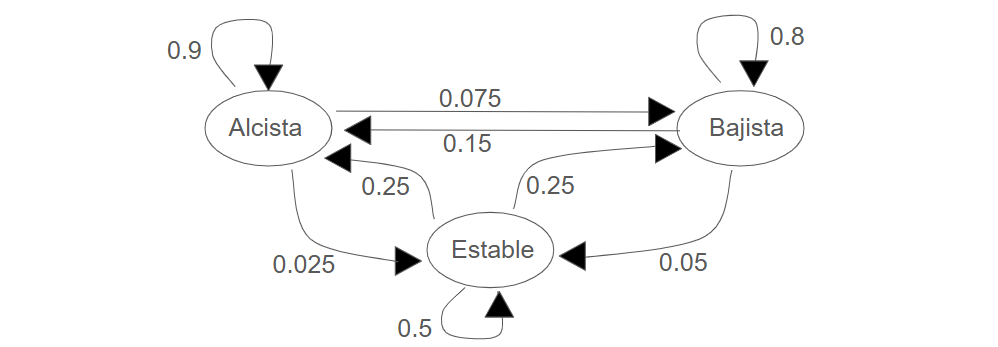
\includegraphics[width=0.8\textwidth]{../Images/Market/Market4.png}
}}
\only<5->{
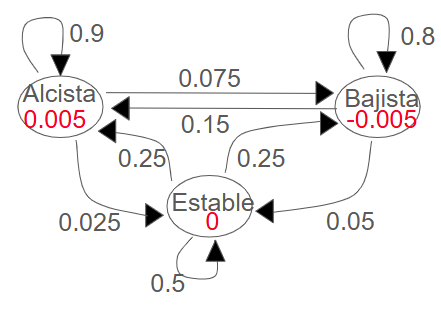
\includegraphics[width=0.45\textwidth]{../Images/Market/MarketWithReward.png}}
\end{center}
\begin{itemize}
\item<6-> \textquestiondown C\'omo definir la funci\'on recompensa en este contexto?
\end{itemize}
\end{itemize}
\end{frame}

\begin{frame}{Función de recompensa}
\begin{itemize}
\item Definimos:
\[
r(x)
\]

\item<2-> Interpreta ganancia o costo en el estado $x$

\item<3-> Ejemplo:
\[
r(\text{Alcista}) = 0.005,\quad
r(\text{Bajista}) = -0.005,\quad
r(\text{Estable}) = 0
\]

\item<4-> Ahora podemos evaluar trayectorias
\end{itemize}
\end{frame}

%------------------------------------------------

\begin{frame}{Proceso con recompensa}
\begin{center}
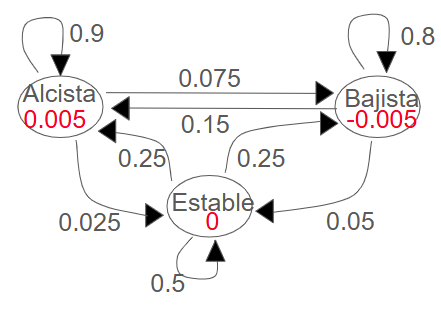
\includegraphics[width=0.45\textwidth]{../Images/Market/MarketWithReward.png}
\end{center}

\begin{itemize}
\item Invertir \$1 → $\$(1+r(x))$ después de una semana
\end{itemize}
\end{frame}

%------------------------------------------------

\begin{frame}{Evaluando una trayectoria}
\begin{itemize}
\item Estados: $x_0, x_1, x_2$

\item<2-> Ganancia total (intereses simples para facilitar):
\[
r(x_0)+r(x_1)+r(x_2)
\]

\item<3-> No conocemos el futuro → usamos valor esperado
\begin{itemize}
\item<3-> Empezando con una semana en estado $x_0$, la ganancia total en 3 semanas ser\'a:
$$
{\rm E}\left[r(x_0)+r(x_1)+r(x_2) | x_0\right]
$$
\item<4->\textquestiondown El valor esperado es con respecto a qu\'e?
\end{itemize}
\end{itemize}
\end{frame}

%------------------------------------------------


%------------------------------------------------

\begin{frame}{Idea central}
\begin{itemize}
\item Queremos evaluar estados considerando el futuro

\item<2-> Definimos la \textbf{función valor}
\begin{itemize}
\item En el ejemplo de reg\'imenes de mercado, captura la ganancia esperada en 3 semanas, dado el estado de la semana actual ($x_0$ = Alcista, Bajista o Estable):
$$
V(x_0) = {\rm E}\left[r(x_0)+r(x_1)+r(x_2) | x_0\right]
$$
\end{itemize}
\item<3-> Intuición:
\begin{itemize}
\item Qué tan bueno es estar en un estado hoy
\end{itemize}
\end{itemize}
\end{frame}

\begin{frame}{Funci\'on Valor - Intuición}
\begin{itemize}
\item Cómo podríamos construir un jugador de ajedrez?
\begin{center}
 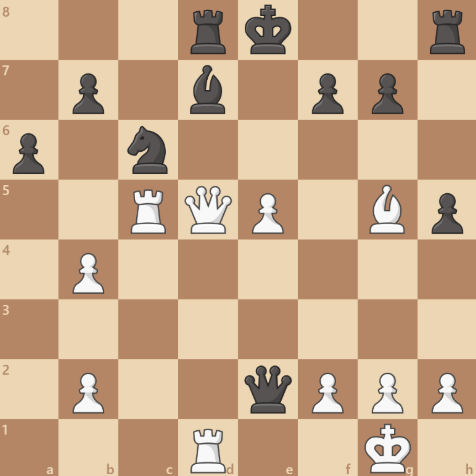
\includegraphics[width=0.5\textwidth]{../Images/Figures/Chess.png}   
\end{center}
\item<2-> Si tuviéramos una función para evaluar la probabilidad de ganar el juego a partir de cada posición, podríamos elegir la mejor acción
\item<3-> Esa función existe y es bien definida para MRPs y MDPs. Se denomina {\bf función valor.}
\end{itemize}
\end{frame}


\begin{frame}{Función valor como tabla}
\begin{itemize}
\item Pensemos la función valor como una tabla.
\item Filas: estados \(x\)
\item Columnas: tiempo \(t\)
\end{itemize}

\begin{center}
\begin{tabular}{|c|c|c|c|}
\hline
\diagbox{$x$}{$t$} & 0 & 1 & 2 \\ \hline
Alcista & ? & ? & ? \\
Bajista & ? & ? & ? \\
Estable & ? & ? & ? \\ \hline
\end{tabular}
\end{center}
$V_t(x)$ = ganancia esperada empezando a partir de la semana $t$, con estado $x$.
\pause
\begin{block}{Idea clave}
Resolver el problema = llenar esta tabla.
\end{block}
\end{frame}

\begin{frame}{Recursión}
\begin{itemize}
\item El concepto de función valor es central para la toma de decisiones secuenciales.
\item<2-|handout> Otro concepto que vamos a utilizar es la idea de {\bf recursión}.
\item<3-|handout> Para eso, vamos a representar el proceso con un nuevo grafo, utilizando el tiempo como segundo eje.
\end{itemize}
\begin{center}
\only<4|presentation>{
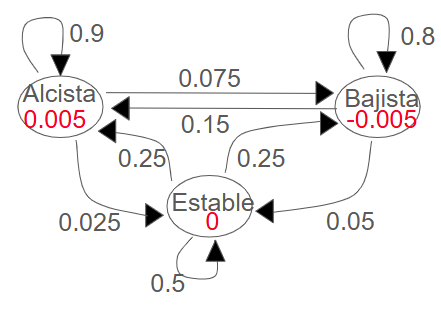
\includegraphics[width=0.8\textwidth]
{../Images/Market/MarketWithReward.png}}
\only<5|presentation>{
\hspace{-1.1cm}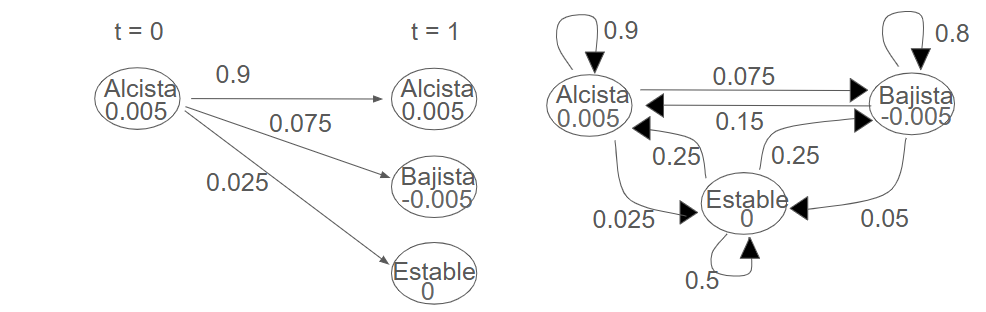
\includegraphics[width=1.1\textwidth]
{../Images/Market/Recursion1.png}}
\only<6|presentation>{
\hspace{-1.1cm}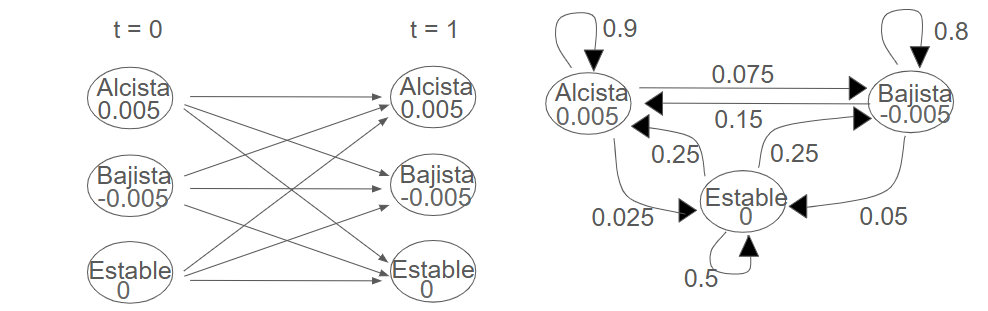
\includegraphics[width=1.1\textwidth]
{../Images/Market/Recursion2.png}}
\only<7-|handout>{
\hspace{-1cm}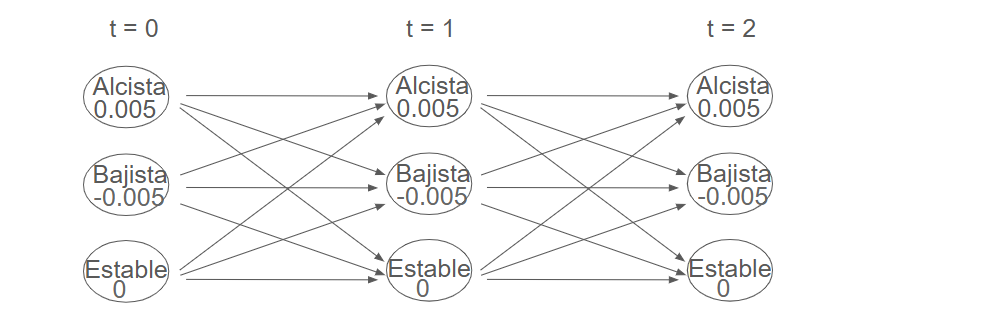
\includegraphics[width=1.1\textwidth]
{../Images/Market/Recursion3.png}}
\end{center}
\only<8-|handout>{\textcolor{red}{Idea: resolver una serie de problemas más fáciles, hasta llegar a la respuesta original.}}
\end{frame}

\begin{frame}{Recursión hacia atrás}
\begin{itemize}
\item Empezamos desde el final.
\end{itemize}

\[
V_2(x) = r(x)
\]

\pause

\begin{itemize}
\item Luego usamos recursión:
\end{itemize}

\[
V_t(x) = r(x) + \sum_y P(x,y)V_{t+1}(y)
\]

\pause

\begin{block}{Idea}
Propagamos valores hacia atrás en el tiempo.
\end{block}
\end{frame}


\begin{frame}{Calculando La Función Valor Por Recursión}
\begin{center}
\mode<beamer>{
\only<1-2>{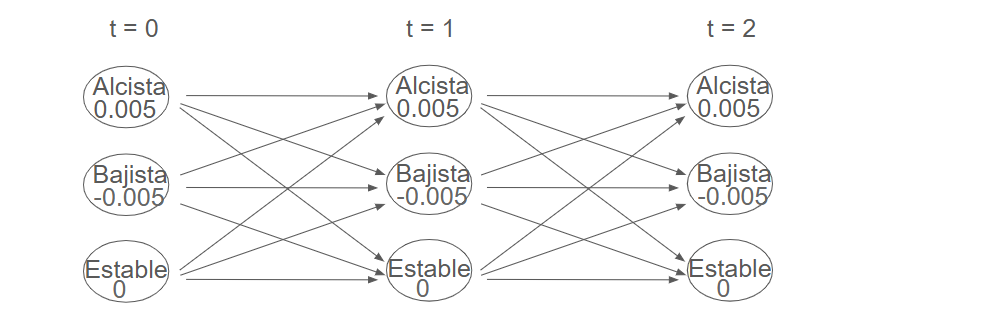
\includegraphics[width=0.8\textwidth]
{../Images/Market/Recursion3.png}}
\only<3-4>{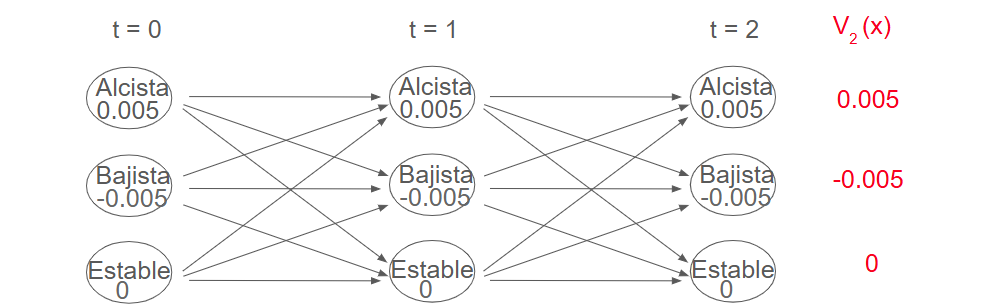
\includegraphics[width=0.8\textwidth]
{../Images/Market/Recursion4.png}}}
\only<5-7>{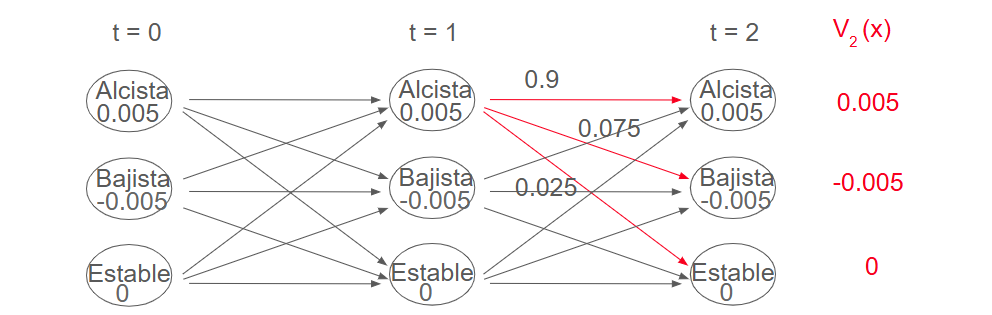
\includegraphics[width=0.8\textwidth]
{../Images/Market/Recursion5.png}}
\mode<beamer>{
\only<8>{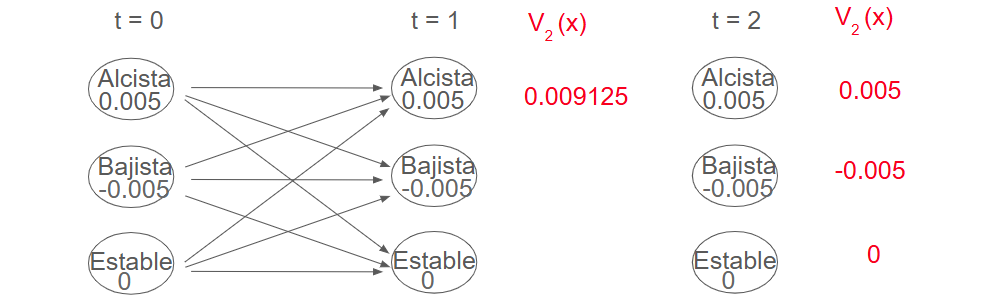
\includegraphics[width=0.8\textwidth]
{../Images/Market/Recursion6.png}}
\only<9-10>{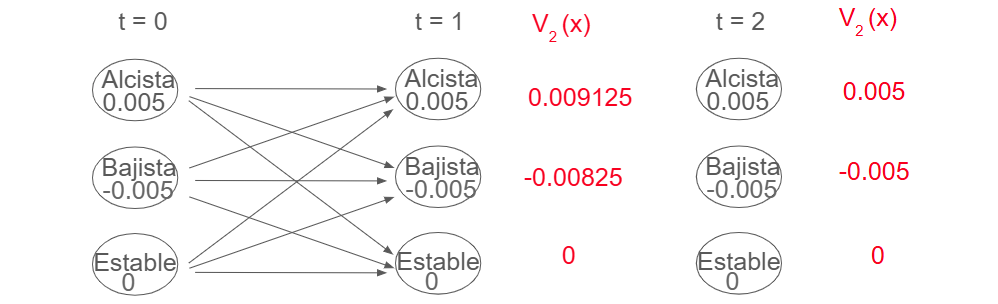
\includegraphics[width=0.8\textwidth]
{../Images/Market/Recursion7.png}}
\only<11->{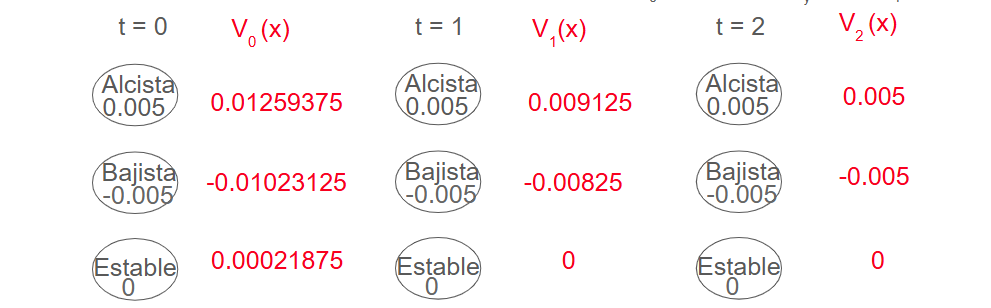
\includegraphics[width=0.8\textwidth]
{../Images/Market/Recursion8.png}}}
\end{center}
$V_t(x)$ = ganancia total esperada empezando en el estado $x$ en tiempo $t$.
\begin{enumerate}
\item<2->Calculamos $V_2(x) = r(x)$.
\item<4->Retrocedemos una semana y calculamos 
$V_1 (x)= r(x)+\sum_y P(x,y)V_2(y)$
\mode<beamer>{\only<5-9>{{\small
$$
\begin{array}{ccl}
V_1(\mathbf{A}) & = & r(\mathbf{A})+ \sum_y P(\mathbf{A},y) V_2(y)\\
\only<6-9> {& = & 0.005+0.9\times 0.005+0.075\times (-0.005)+0.025\times 0\\}
\only<7-9> {& = & 0.009125}
\end{array}
$$
}}

\only<9> {Repetimos el mismo procedimiento con $x=\mathbf{Bajista}$ y $x=\mathbf{Estable}$.}}
\item<10-> Retrocedemos otra semana y calculamos $V_0(x) = r(x) + \sum_yP(x,y)V_1(y).$
\end{enumerate}
\end{frame}

\begin{frame}{La Funci\'on Valor}
\begin{itemize}
\item Con esos c\'alculos, tenemos:
\begin{tabular}{|c|c|c|c|} \hline
\diagbox{$x$}{$t$} & 0 & 1 & 2 \\ \hline
Alcista & 0.01259375 & 0.009125 & 0.005 \\ \hline
Bajista & -0.01023125 & -0.00825 &-0.005 \\ \hline 
Estable & 0.00021875 & 0 & 0 \\ \hline
\end{tabular}
\item<2-> Interpretaci\'on:
\begin{itemize}  
\item<3-> $V_0(\text{Alcista}) = 0.01259375$ $\mapsto$ si la semana actual es alcista, esperamos ganancia de
\textcolor{red}{0.01259375 en 3 semanas}  
\item<3-> $V_1(\text{Bajista}) = -0.00825$ $\mapsto$ si la semana actual es bajista, esperamos p\'erdida de
\textcolor{red}{0.00825 en 2 semanas}
\end{itemize}
\end{itemize}
\end{frame}

\begin{frame}{Generalizando hasta ac\'a: MRP}
\begin{itemize}
\item Proceso markoviano con recompensa definido por la tupla $(S,P,r)$
\item<2-> Distintas maneras de combinar $r(x_t),~t=0,1,\dots$ en un único criterio (suma, multiplicación, medidas de riesgo)
\item<3->Una de las definiciones más comúnmente utilizadas es la recompensa total:
$$
V_t(x) = {\rm E}\left[\sum_{\tau=t}^T r(x_\tau)|x_t = x\right]$$
\begin{itemize}
\item $T$ es el \textbf{horizonte} (finito)
\end{itemize}
\end{itemize}
\end{frame}

\begin{frame}{Generalizando hasta ac\'a: Recursi\'on}
\begin{itemize}
\item Definimos Vt(x) recursivamente:
{\small $$
\begin{array}{ccl}
V_T(x) & = & r(x) \\
V_t(x) & = & r(x) +  \sum\limits_y P(x,y) V_{t+1}(y) 
\end{array}
$$}
\item<4-> Podemos usar notación de matrices para simplificar las ecuaciones:
$$
\begin{array}{ccl}
V_T &=& r \\
V_t & = & r+ P V_{t+1},~t = 0,...,T-1
\end{array}
$$
donde $r \in \Re^{|S|}$, $V_t \in \Re^{|S|}$, $P \in \Re^{|S|\times|S|}$.
\item<5-> Podemos implementar el algoritmo en Python.
\end{itemize}
\end{frame}

\begin{frame}{Observaciones}
\begin{itemize}
\item Asumimos que $r$ y $P$ no dependen de $t$, entonces el proceso markoviano es homogéneo en el tiempo. Pero se puede extender el resultado al caso en que dependen de $t$: 
$$
\begin{array}{ccl}
V_T &=& r_T \\
V_t & = & r_t+ \alpha P_t V_{t+1},~t = 0,...,T-1
\end{array}
$$
\item<2-> También asumimos que la recompensa es determinística, pero podemos incorporar casos en que es aleatoria:                $$
\bar{r}(x) = {\rm E}_w\left[r(x,w)\right]
$$                          
\item<3-> Si la recompensa depende del próximo estado además del actual, también se puede incorporar utilizando: 
$$
\bar{r}(x) = {\rm E}\left[r(x,x_{t+1})| x_t = x\right] = \sum_y P(x,y)r(x,y)
$$ 
\end{itemize}
\end{frame}

\begin{frame}{Ejemplo: gestión de inventario}

\begin{center}
\large
¿Cómo decidir cuánto stock mantener al largo del tiempo?
\end{center}

\pause

\begin{itemize}
\item La demanda es incierta
\item Las decisiones hoy afectan el futuro
\item \textquestiondown Qu\'e costos est\'an involucrados?
\end{itemize}
\end{frame}

\begin{frame}{Descripción del problema}

En cada período \(t = 0,1,\dots,T\):

\begin{itemize}
\item Tenemos un nivel de inventario
\item Ocurre una demanda aleatoria
\item El inventario cambia
\end{itemize}

\pause

\begin{center}
\Large
¿Qué necesitamos modelar?
\end{center}

\end{frame}

\begin{frame}{¿Cuál debería ser el estado?}

\textbf{Primera opción:}
\begin{itemize}
\item Solo el inventario actual
\[
X_t = \text{inventario en } t
\]
\end{itemize}

\pause

\textbf{Pregunta:} ¿esto siempre alcanza?

\pause

\textbf{Si la demanda es completamente aleatoria:}
\begin{itemize}
\item Sí, el inventario resume toda la información relevante
\end{itemize}

\pause

\textbf{Si la demanda tiene patrón (ej: estacionalidad):}
\begin{itemize}
\item Tal vez necesitamos incluir:
\begin{itemize}
\item el tiempo \(t\)
\item o una variable de “estado de demanda”
\end{itemize}
\end{itemize}

\end{frame}

\begin{frame}{Espacio de estados}

Supongamos:

\[
S = \{0,1,2,\dots,N\}
\]

\pause

\begin{itemize}
\item \(0\): sin stock
\item \(N\): capacidad máxima
\end{itemize}

\pause

\textbf{Interpretación:}
\begin{itemize}
\item Estado = unidades disponibles
\end{itemize}

\end{frame}

\begin{frame}{¿Cómo evoluciona el sistema?}

\textbf{Demanda aleatoria:}
\[
D_t \sim \text{Distribución conocida}
\]

\pause

\textbf{Transición:}
\[
X_{t+1} = 
\begin{cases} 
X_t - D_t & \text{ if } X_t - D_t \geq n  \\
N & \text{ if } X_t - D_t < n 
\end{cases}
\]

\pause

\textbf{Hoy:} las decisiones est\'an fijas, volver al nivel m\'aximo $N$ si el nivel queda por debajo de un l\'imite $n$.

\end{frame}
\begin{frame}{Probabilidades de transición}

Recordemos la dinámica:

\[
X_{t+1} = 
\begin{cases} 
X_t - D_t & \text{si } X_t - D_t \geq n \\[4pt]
N & \text{si } X_t - D_t < n 
\end{cases}
\]

\pause

Queremos calcular:

\[
P_{ij} = \mathbb{P}(X_{t+1} = j \mid X_t = i)
\]

\pause

\textbf{Caso 1: transición sin reposición (\(j \geq n\))}

\[
P_{ij} = \mathbb{P}(D_t = i - j), \quad \text{para } j \in \{n, \dots, i\}
\]

\pause

\textbf{Caso 2: reposición a \(N\)}

\[
P_{iN} = \mathbb{P}(X_t - D_t < n)
= \mathbb{P}(D_t > i - n)
\]

\pause

\textbf{En otro caso:}

\[
P_{ij} = 0
\]

\end{frame}

\begin{frame}{¿Cómo definimos la recompensa?}

\textbf{Opciones comunes:}

\pause

\begin{itemize}
\item Ingresos por ventas
\item Costo de mantener inventario
\item Penalización por faltantes
\end{itemize}

\pause

\textbf{Ejemplo:}

\[
r(i) = \text{beneficio esperado en estado } i
\]

\pause

\textbf{Pregunta:}
\begin{itemize}
\item ¿depende solo del estado?
\item ¿o también de la demanda realizada?
\end{itemize}

\end{frame}

\begin{frame}{Ejemplo de recompensa}

Una posible definición:

\[
r(i) = \mathbb{E}[\text{ventas} - \text{costos} \mid X_t = i]
\]

\pause

Ejemplo simple:

\[
r(i) = p \cdot \mathbb{E}[\min(i, D_t)] - c \cdot i
\]

\pause

\begin{itemize}
\item \(p\): precio
\item \(c\): costo de holding
\end{itemize}

\end{frame}

\begin{frame}{Horizonte}

\textbf{Horizonte finito:}
\[
t = 0,1,\dots,T
\]

\pause

\textbf{Interpretación:}
\begin{itemize}
\item Problema de planificación a \(T\) períodos
\end{itemize}

\pause

\textbf{Alternativa:}
\begin{itemize}
\item horizonte infinito (más adelante)
\end{itemize}

\end{frame}

\begin{frame}{Modelo como MRP}

Tenemos:

\begin{itemize}
\item Estados: \(S = \{0,\dots,N\}\)
\item Transiciones: \(P_{ij}\)
\item Recompensas: \(r(i)\)
\item Horizonte: \(T\)
\end{itemize}

\pause

\begin{center}
\Large
¡Es un Markov Reward Process!
\end{center}

\end{frame}

\begin{frame}{Extensión natural}

\begin{center}
\Large
¿Y si pudiéramos decidir cuánto reponer?
\end{center}

\pause

\begin{itemize}
\item Aparece una acción \(U_t\)
\item Cambian las transiciones
\item Cambian las recompensas
\end{itemize}

\pause

\begin{center}
\Large
→ Markov Decision Process (MDP)
\end{center}

\end{frame}

\end{document}